\documentclass{article}

\usepackage{graphicx}
\usepackage[hidelinks]{hyperref}
\usepackage{geometry}
\usepackage{amsmath}
\usepackage{listings}
\usepackage{wrapfig}
\usepackage{subcaption}
\usepackage{tikz}
\usetikzlibrary{positioning}

\geometry{
 a4paper,
 left=20mm,
 right=20mm,
 top=20mm,
 bottom=25mm,
}

\begin{document}

\begin{titlepage}
\begin{center}
\vspace*{1cm}
            
\Huge
\textbf{Midterm Project}
            
\vspace{1cm}

\Large
\text{Due: Sunday, October 27, 2024}

\vspace{2cm}

\text{\texttt{Brian High}} \\
\text{\texttt{Thomas Hynes}} \\
\text{\texttt{Jeremy Middleman}} \\
\text{\texttt{Andrei Phelps}} \\
\text{\texttt{Wayne Rudnick}} \\

\vspace{2cm}

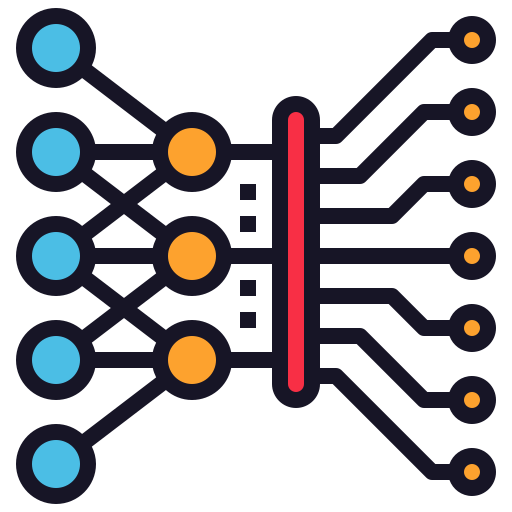
\includegraphics[scale=0.25]{figs/icon.png}\\[0.5cm]

\vspace{9cm}

\textbf{CS 491/591: Neural Networks} \\

\end{center}
\end{titlepage}
\newpage

\section{Feedforward Neural Network (FNN)}

\subsection{Data Structures for FNN}

\subsubsection{\textbf{Layers}}
The FNN is composed of multiple layers stored as a list of layer objects within the network. Each layer object encapsulates essential information, including its weights, activation function, and gradient values, making it easy to process data through multiple layers.

\begin{itemize}
    \item \textbf{Weights}: Each layer contains weights stored as a matrix, initialized with random values. The weights include an additional column to accommodate the bias term, ensuring consistent results in the forward pass.
    \item \textbf{Activation Functions}: Each layer applies an activation function to the weighted input, introducing non-linearity into the model. The activations used include sigmoid, logsoftmax, and identity functions.
    \item \textbf{Gradients}: Gradients for each weight are accumulated in each layer, allowing the model to perform weight updates after each mini-batch.
\end{itemize}

\subsection{Forward and Backward Propagation}

\subsubsection{Forward Pass}
The forward pass involves feeding input data sequentially through each layer in the network. For each layer:
\begin{itemize}
    \item The layer calculates the dot product of its inputs and weights, then adds a bias term.
    \item The result is passed through an activation function, introducing non-linearity into the model.
    \item The activated output becomes the input for the next layer.
\end{itemize}
\begin{figure}[h!]
    \centering
    \resizebox{0.5\linewidth}{!}{ % Adjusts the size to half the linewidth while maintaining aspect ratio
    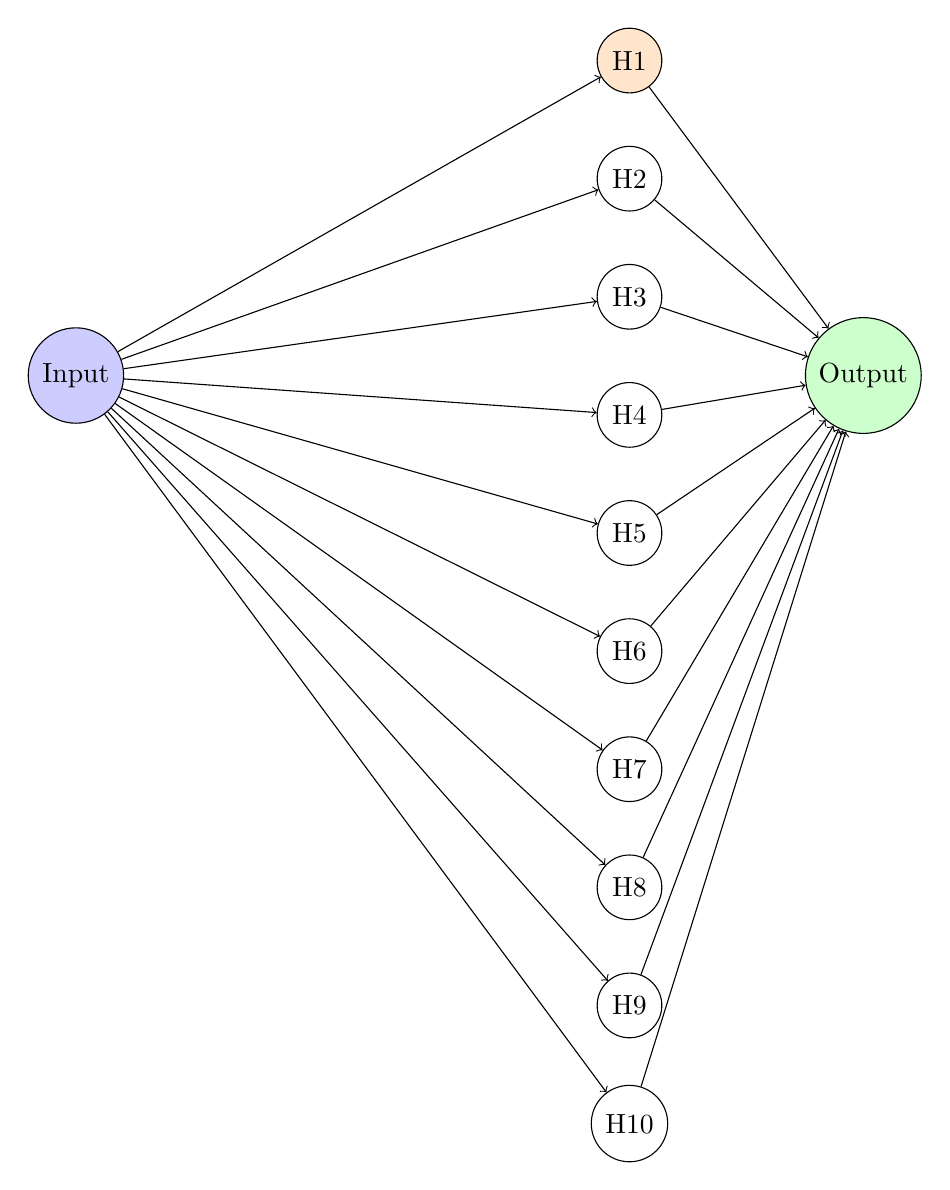
\begin{tikzpicture}

        % Define layer node style
        \tikzstyle{neuron} = [circle, draw, minimum size=0.8cm, node distance=1.5cm]

        % Input Layer
        \node[neuron, fill=blue!20] (input) at (0,0) {Input};

        % Hidden Layer (10 Neurons)
        \node[neuron, right=of input, xshift=4.5cm, yshift=4cm, fill=orange!20] (hidden1) {H1};
        \node[neuron, below of=hidden1] (hidden2) {H2};
        \node[neuron, below of=hidden2] (hidden3) {H3};
        \node[neuron, below of=hidden3] (hidden4) {H4};
        \node[neuron, below of=hidden4] (hidden5) {H5};
        \node[neuron, below of=hidden5] (hidden6) {H6};
        \node[neuron, below of=hidden6] (hidden7) {H7};
        \node[neuron, below of=hidden7] (hidden8) {H8};
        \node[neuron, below of=hidden8] (hidden9) {H9};
        \node[neuron, below of=hidden9] (hidden10) {H10};

        % Output Layer
        \node[neuron, fill=green!20] (output) at (10,0) {Output};

        % Draw arrows from Input Layer to Hidden Layer
        \foreach \i in {1,...,10}
            \draw[->] (input) -- (hidden\i);

        % Draw arrows from Hidden Layer to Output Layer
        \foreach \i in {1,...,10}
            \draw[->] (hidden\i) -- (output);

    \end{tikzpicture}
    }
    \caption{Data Flow Through the Network During the Forward Pass}
\end{figure}
During the forward pass, each input is passed through the network’s layers sequentially. Each layer computes the dot product of its inputs and weights, applies the activation function, and passes the result to the next layer.


\subsubsection{Backward Pass (Backpropagation)}
The backward pass, or backpropagation, calculates gradients for each layer’s weights, enabling the network to minimize the loss function. In this process:
\begin{itemize}
    \item The derivative of the loss function with respect to the network's output is computed.
    \item Each layer computes the gradient of its weights based on this derivative, the layer's inputs, and the activation function's derivative.
    \item These gradients are accumulated across the mini-batch and used to update the weights during gradient descent.
\end{itemize}

\section{Data Organization in Backpropagation}

Backpropagation is implemented using a gradient descent algorithm over mini-batches of data, which allows efficient updates after each batch. Gradients for the weights are computed by first calculating the derivative of the loss function with respect to the network’s output. Each layer then computes its weight gradients based on its inputs and these derivatives, storing the gradients in an accumulator for weight updates. Once a mini-batch is processed, the weights are updated based on the accumulated gradients.

\section{Experiments and Results}

\subsection{Sinusoidal Regression}
In the sinusoidal regression experiment, the FNN was trained to approximate the function $y = \sin(x)$ using a single hidden layer of 10 neurons. The network's approximation was observed to converge towards the sine function, indicating that the FNN effectively learned the relationship. Our tests showed that the results were almost perfect at about 1000,000 epochs.

\begin{figure}[h!]
    \centering
    % First row of images
    \begin{subfigure}{0.45\textwidth}
        \centering
        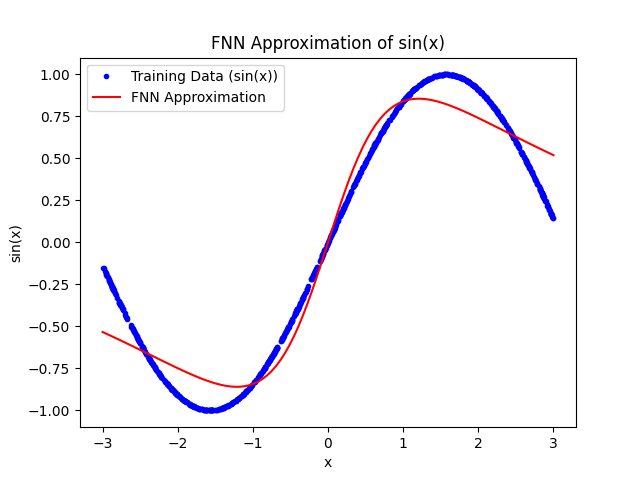
\includegraphics[width=\linewidth]{figs/FNN_Test01.png}
        \caption*{Approximation After 100 Epochs}
        \label{fig:100epochs}
    \end{subfigure}
    \hfill
    \begin{subfigure}{0.45\textwidth}
        \centering
        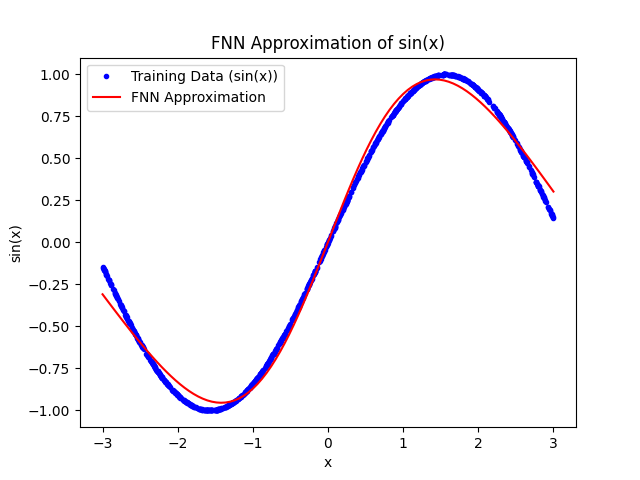
\includegraphics[width=\linewidth]{figs/FNN_Test02.png}
        \caption*{Approximation After 1,000 Epochs}
        \label{fig:1000epochs}
    \end{subfigure}

    % Second row of images
    \begin{subfigure}{0.45\textwidth}
        \centering
        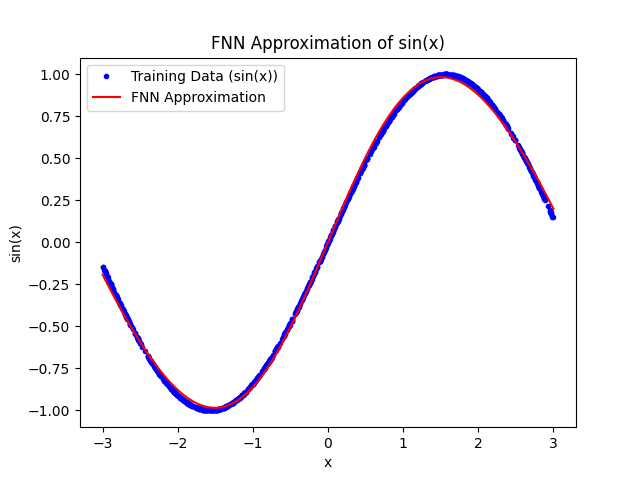
\includegraphics[width=\linewidth]{figs/FNN_Test03.png}
        \caption{Approximation After 10,000 Epochs}
        \label{fig:10000epochs}
    \end{subfigure}
    \hfill
    \begin{subfigure}{0.45\textwidth}
        \centering
        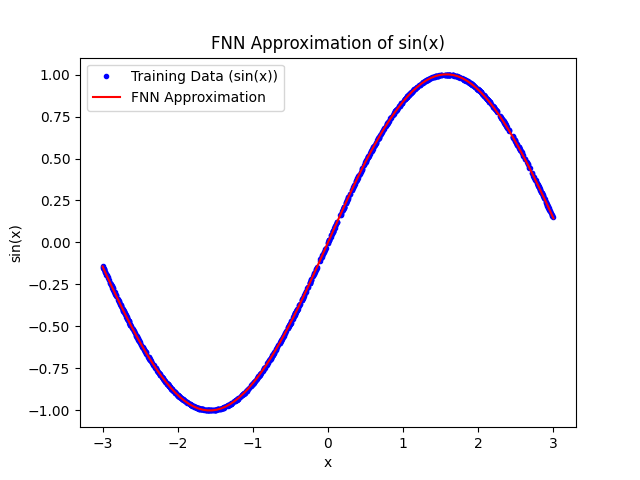
\includegraphics[width=\linewidth]{figs/FNN_Test04.png}
        \caption*{Approximation After 100,000 Epochs}
        \label{fig:finalapproximation}
    \end{subfigure}
    \label{fig:sin_approximation}
\end{figure}

\subsection{Data-Driven Model for ODE}
The data-driven model was tested using the Van der Pol oscillator’s differential equations. Two different differential equations were tested to compare the effects of varying the data. The results showed distinct patterns, as shown below.

\begin{figure}[h!]
    \centering
    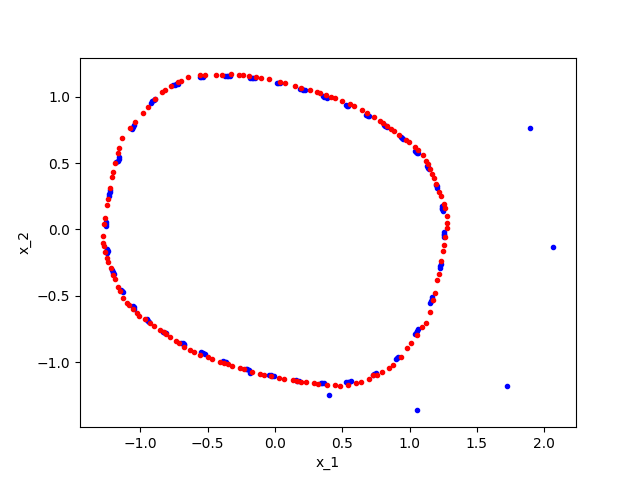
\includegraphics[scale=0.4]{figs/Vander_Test01.png}
    \caption{Data-driven model using the ODE from the assignment (800 epochs).}
\end{figure}

\begin{figure}[h!]
    \centering
    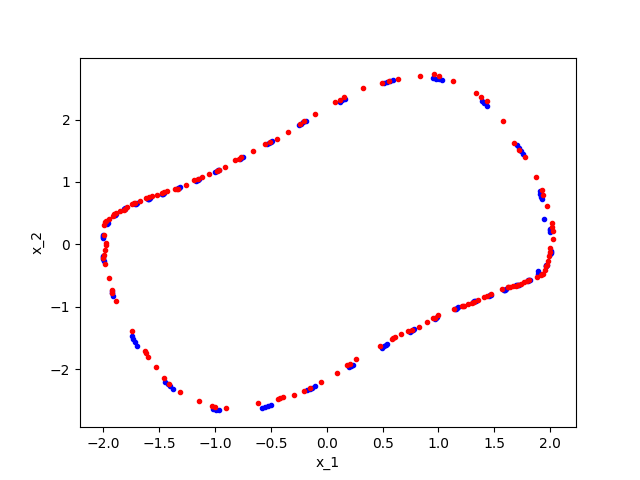
\includegraphics[scale=0.4]{figs/Vander_Test02.png}
    \caption{Data-driven model using the Van der Pol ODE from the provided file (800 epochs).}
\end{figure}

\subsection{Handwritten Digit Classification}

The MNIST dataset was used to test the FNN on handwritten digit classification. The network achieved significant accuracy, showing its capability to handle complex datasets and make reliable predictions.

\section{Individual Contributions}

\subsection{Brian High}
\begin{itemize}
    \item[1)] 
\end{itemize}

\subsection{Thomas Hynes}
\begin{itemize}
    \item[1)] 
\end{itemize}

\subsection{Jeremy Middleman}
\begin{itemize}
    \item[1)] 
\end{itemize}

\subsection{Andrei Phelps}
\begin{itemize}
    \item[1)] 
\end{itemize}

\subsection{Wayne Rudnick}
\begin{itemize}
    \item[1)] 
\end{itemize}

\end{document}
